\documentclass[12pt,a4paper]{article}

% for polish language
\usepackage{polski}

% for some math symbols
\usepackage{amssymb}

% correct footnotes placement
\usepackage[bottom]{footmisc}

% for \say command
\usepackage{dirtytalk}

% change title of the bibliography
\def\bibname{Referencje}\let\refname\bibname

% for advanced math formulas
\usepackage{mathtools}

\usepackage{listings}
% colors for snippet background
\usepackage{xcolor}

% links
\usepackage{hyperref}
% \hypersetup{
%     colorlinks,
%     citecolor=black,
%     filecolor=black,
%     linkcolor=black,
%     urlcolor=blue
% }

% image displaying
\usepackage{subcaption}
\usepackage{graphicx}

\usepackage{multirow} 
\usepackage{makecell}

% display structure of the project
\usepackage{dirtree}

% include pdf images
\usepackage{pdfpages}

\title{Dokumentacja do projektu z AMHE}

\author{Roman Moskalenko \and Pavel Tarashkevich}
\date{}

\begin{document}

\maketitle

\section{Treść zadania}

\textbf{Zadanie 10.}\\

Zaprojektuj algorytm ewolucyjny i zbadaj jego działanie w jednym z zadań zdefiniowanych w ramach środowiska OpenAI poświęconym kontroli.

Specyfikacja zadań znajduje się pod poniższym linkiem:

\href{https://gym.openai.com/envs/#classic\_control}{gym.openai.com/envs/\#classic\_control}

Porównaj wyniki swojego rozwiązania z dwoma wybranymi rozwiązaniami, które bazują na
innych podejściach.


\section{Projekt wstępny}

\subsection{Opis problemu i jego sposób rozwiązania}

Zadania kontroli klasycznej zakładają sterowanie obiektu fizycznego w sposób,
jak najbardziej efektywny dla jego stanu. Funkcja sterowania może być bardzo
skomplikowana, uciążliwe jest jej zaprojektowanie w sposób ręczny.

Algorytmy uczenia się ze wzmocnieniem (dalej RL) są wykorzystywane w zadaniach związanych z kontrolą.
Do ewaluacji tych algorytmów powstał zestaw środowisk OpenAI gym.

Alternatywnym podejściem do zadań kontroli jest bezpośrednie stosowanie sieci
neuronowych, m.i. podejście neuroewolucji zastosowane w \cite{scalable_alternative},
które zakłada połączenie sieci neuronowych i algorytmów ewolucyjnych.

Do rozwiązania tego problemu planujemy zastosować sieć MLP, gdzie wejściem sieci
będzie stan rozważanego środowiska, a wyjściem będzie akcja do wyboru przez agenta.
Sieć ta będzie optymalizowana za pomocą algorytmu ewolucyjnego CMA-ES.

\subsection{Planowane eksperymenty numeryczne}

W ramach eksperymentów ocenimy działanie implementacji naszego algorytmu
neuroewolucji na różnych środowiskach OpenAI gym.

Następnie porównamy jego działanie z dwoma algorytmami RL pod kątem
końcowej nagrody oraz czasu uczenia algorytmu. Wybrane przez nas
algorytmy RL to A2C oraz PPO.


\subsection{Biblioteki wybrane do realizacji projektu}

\begin{itemize}
  \item \textbf{\href{https://github.com/openai/gym}{gym}} - liczne środowiska, w tym kontroli klasycznej,
        do trenowania agentów.
  \item \textbf{\href{https://github.com/CyberAgentAILab/cmaes}{cmaes}} -
        implementacja algorytmu CMA-ES.
  \item \textbf{\href{https://github.com/DLR-RM/stable-baselines3}{stable-baselines}} -
        biblioteka zawierająca gotowe implementację algorytmów RL.
\end{itemize}

\pagebreak
\section{Project końcowy}

\subsection{Opis struktury projektu}

Na rysunku \ref{fig:dirtree} pokazana jest struktura projektu.

\begin{figure}[!ht]
  \dirtree{%
    .1 ..
    .2 .gitignore.
    .2 docs.
    .3 amhe\_docs.tex.
    .2 main.py.
    .2 requirements.txt.
    .2 src.
    .3 cmaes\_nn.py.
    .3 env\_info.py.
    .3 log\_utils.py.
    .3 nn.py.
    .2 test.
    .3 test\_cmaes\_nn.py.
    .3 test\_data.
    .4 example\_log\_a2c.txt.
    .4 example\_log\_cmaesnn.txt.
    .3 test\_log\_extraction.py.
    .3 test\_log\_utils.py.
    .3 test\_nn.py.
  }
  \caption{Struktura plików projektu}
  \label{fig:dirtree}
\end{figure}

Plik \textbf{main.py} odpowiada za główny skrypt, który wykonuje uczenie
modeli oraz zapisanie wyników uczenia: logów oraz wytrenowanych modeli
do katalogów \textbf{.data/logs} oraz \textbf{.data/models} odpowiednio. \\

Kod źródłowy projektu, z którego jest zbudowany \textbf{main.py} znajduje się
w katalogu \textbf{src}:
\begin{itemize}
  \item \textbf{cmaes\_nn.py} - zawiera implementację algorytmu do rozwiązywania
        problemów kontroli klasycznej, jego interfejs jest zbliżony
        do algorytmów RL z pakietu \textbf{stable-baselines3}
        (tzn. posiada implementacje funkcji \emph{learn()}, \emph{predict()},
        \emph{load()}, \emph{save()}). \\
        Łączy w sobie stosowanie algorytmu CMA-ES oraz perceptronu wielowarstwowego.

  \item \textbf{env\_info.py} - zawiera listę nazw środowisk do problemów kontroli
        klasycznej oraz informacje o tym, czy typ akcji jest ciągły bądź dyskretny.

  \item \textbf{log\_utils.py} - zawiera funkcje pomocnicze do przetwarzania
        logów programu.

  \item \textbf{nn.py} - zawiera funkcje do zbudowania perceptronu
        wielowarstwowego, a także funkcje do przypisania wektora parametrów
        do wag perceptronu.
\end{itemize}

Wraz z implementacją projektu powstawały testy do sprawdzenia poprawności
jego działania. Znajdują się w katalogu \textbf{test}. \\

Katalog \textbf{docs} przechowuje dokumentację projektu.
Plik \textbf{requirements.txt} zawiera listę wymaganych do zainstalowania
bibliotek.

\subsection{Uruchomienie projektu}

Dla uruchomienia projektu niezbędne jest posiadania interpretera Python wersji co najmniej 3.8
oraz zainstalowanie bibliotek znajdujących w pliku \textbf{requirements.txt}:

\begin{lstlisting}[
  backgroundcolor = \color{lightgray},
  language=bash,
]
  $ pip install -r requirements.txt
\end{lstlisting}

\bigskip

Następnie można uruchomić główny skrypt za pomocą polecenia:

\begin{lstlisting}[
  backgroundcolor = \color{lightgray},
  language=bash,
]
  $ python main.py
\end{lstlisting}

Testy można uruchomić poleceniem:

\begin{lstlisting}[
  backgroundcolor = \color{lightgray},
  language=bash,
]
  $ python -m unittest discover test
\end{lstlisting}

\pagebreak
\begin{thebibliography}{9}
  \bibitem{scalable_alternative}
  Tim Salimans, Jonathan Ho, Xi Chen, Szymon Sidor, Ilya Sutskever,\\
  Evolution Strategies as a Scalable Alternative to Reinforcement Learning,
  2017, \href{https://arxiv.org/pdf/1703.03864v1.pdf}{https://arxiv.org/pdf/1703.03864v1.pdf}

\end{thebibliography}

\pagebreak
\appendix
\section{Wykresy uczenia algorymów}

\begin{figure}[ht!]
  \centering
  \begin{subfigure}[ht!]{0.35\textwidth}
    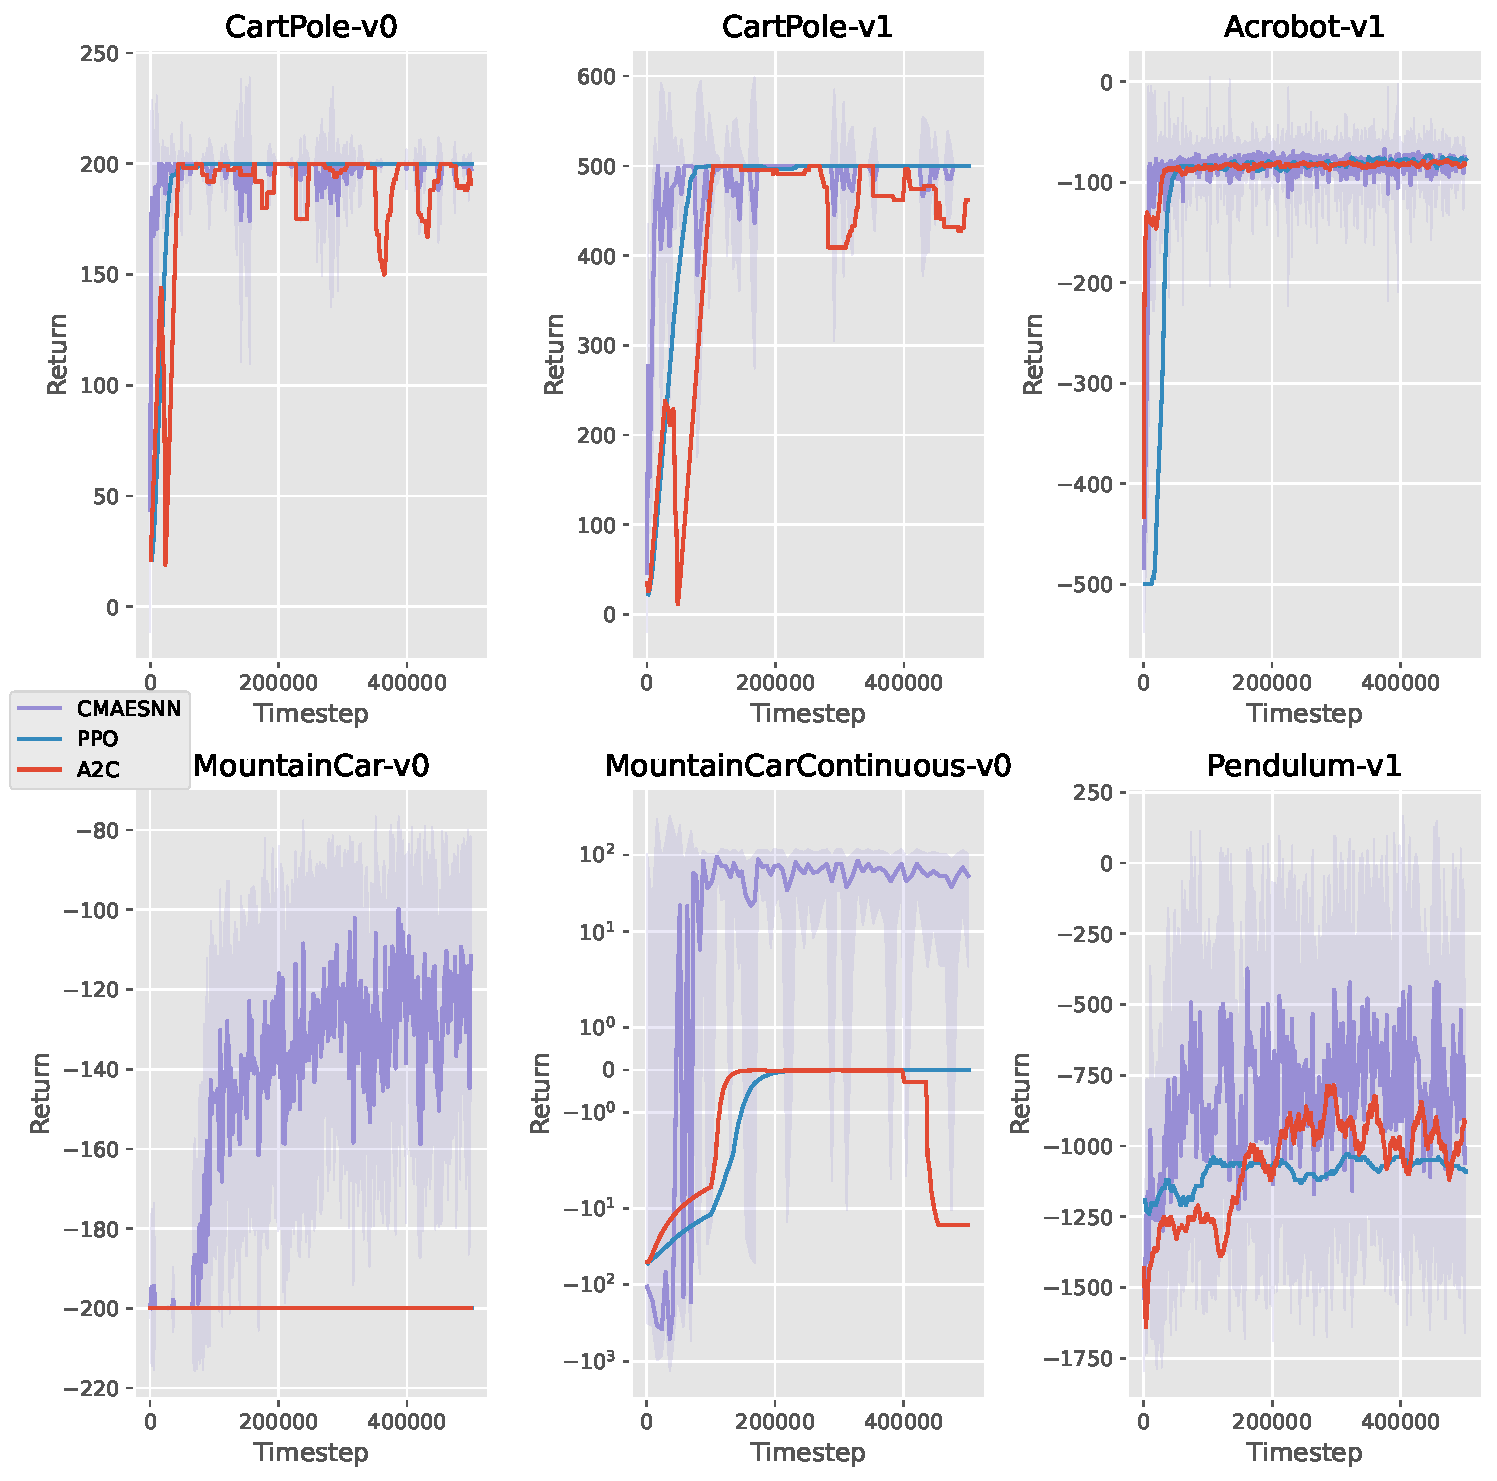
\includegraphics[width=\textwidth]{../plotting/plots/plot_all0.pdf}
    \caption{}
  \end{subfigure}
  \hspace{0.05\textwidth}
  \begin{subfigure}[ht!]{0.35\textwidth}
    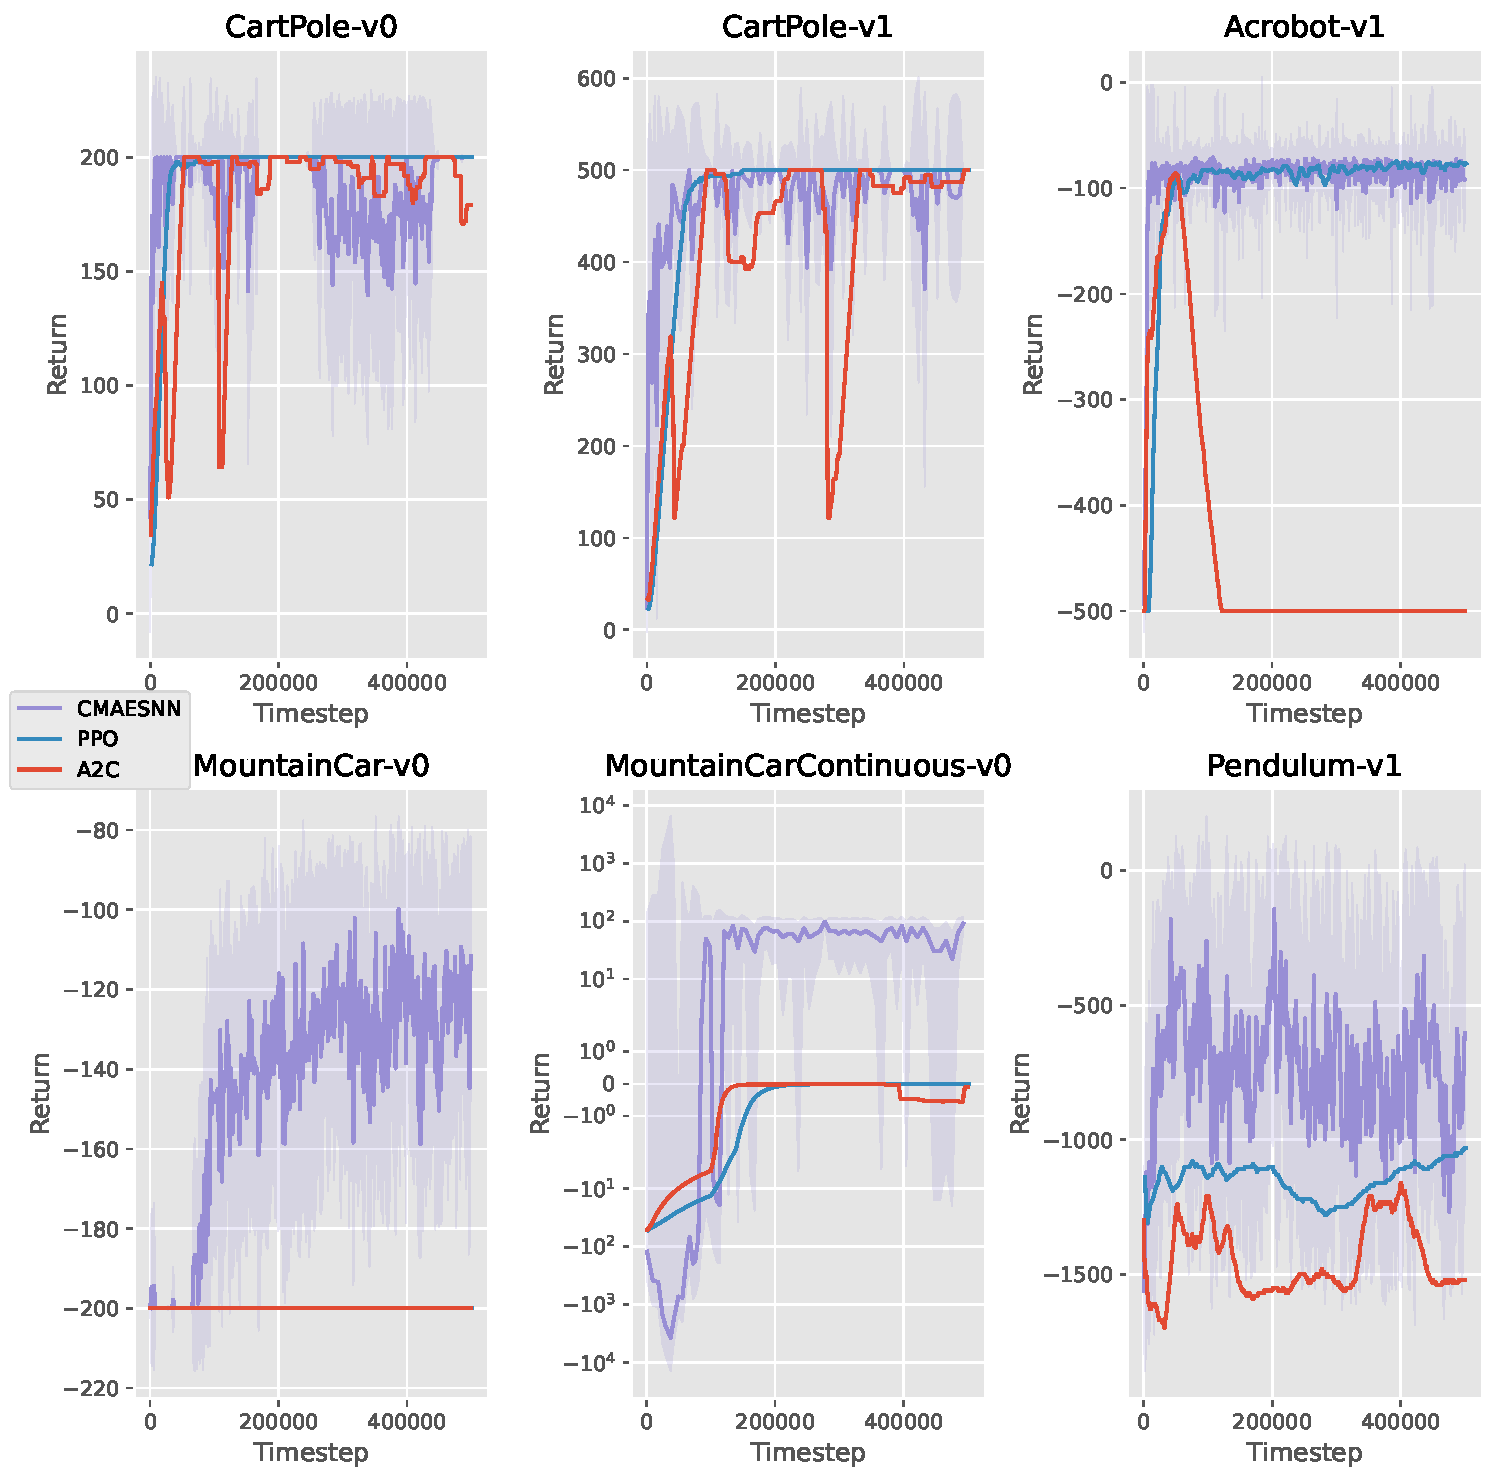
\includegraphics[width=\textwidth]{../plotting/plots/plot_all1.pdf}
    \caption{}
  \end{subfigure}

  \begin{subfigure}[ht!]{0.35\textwidth}
    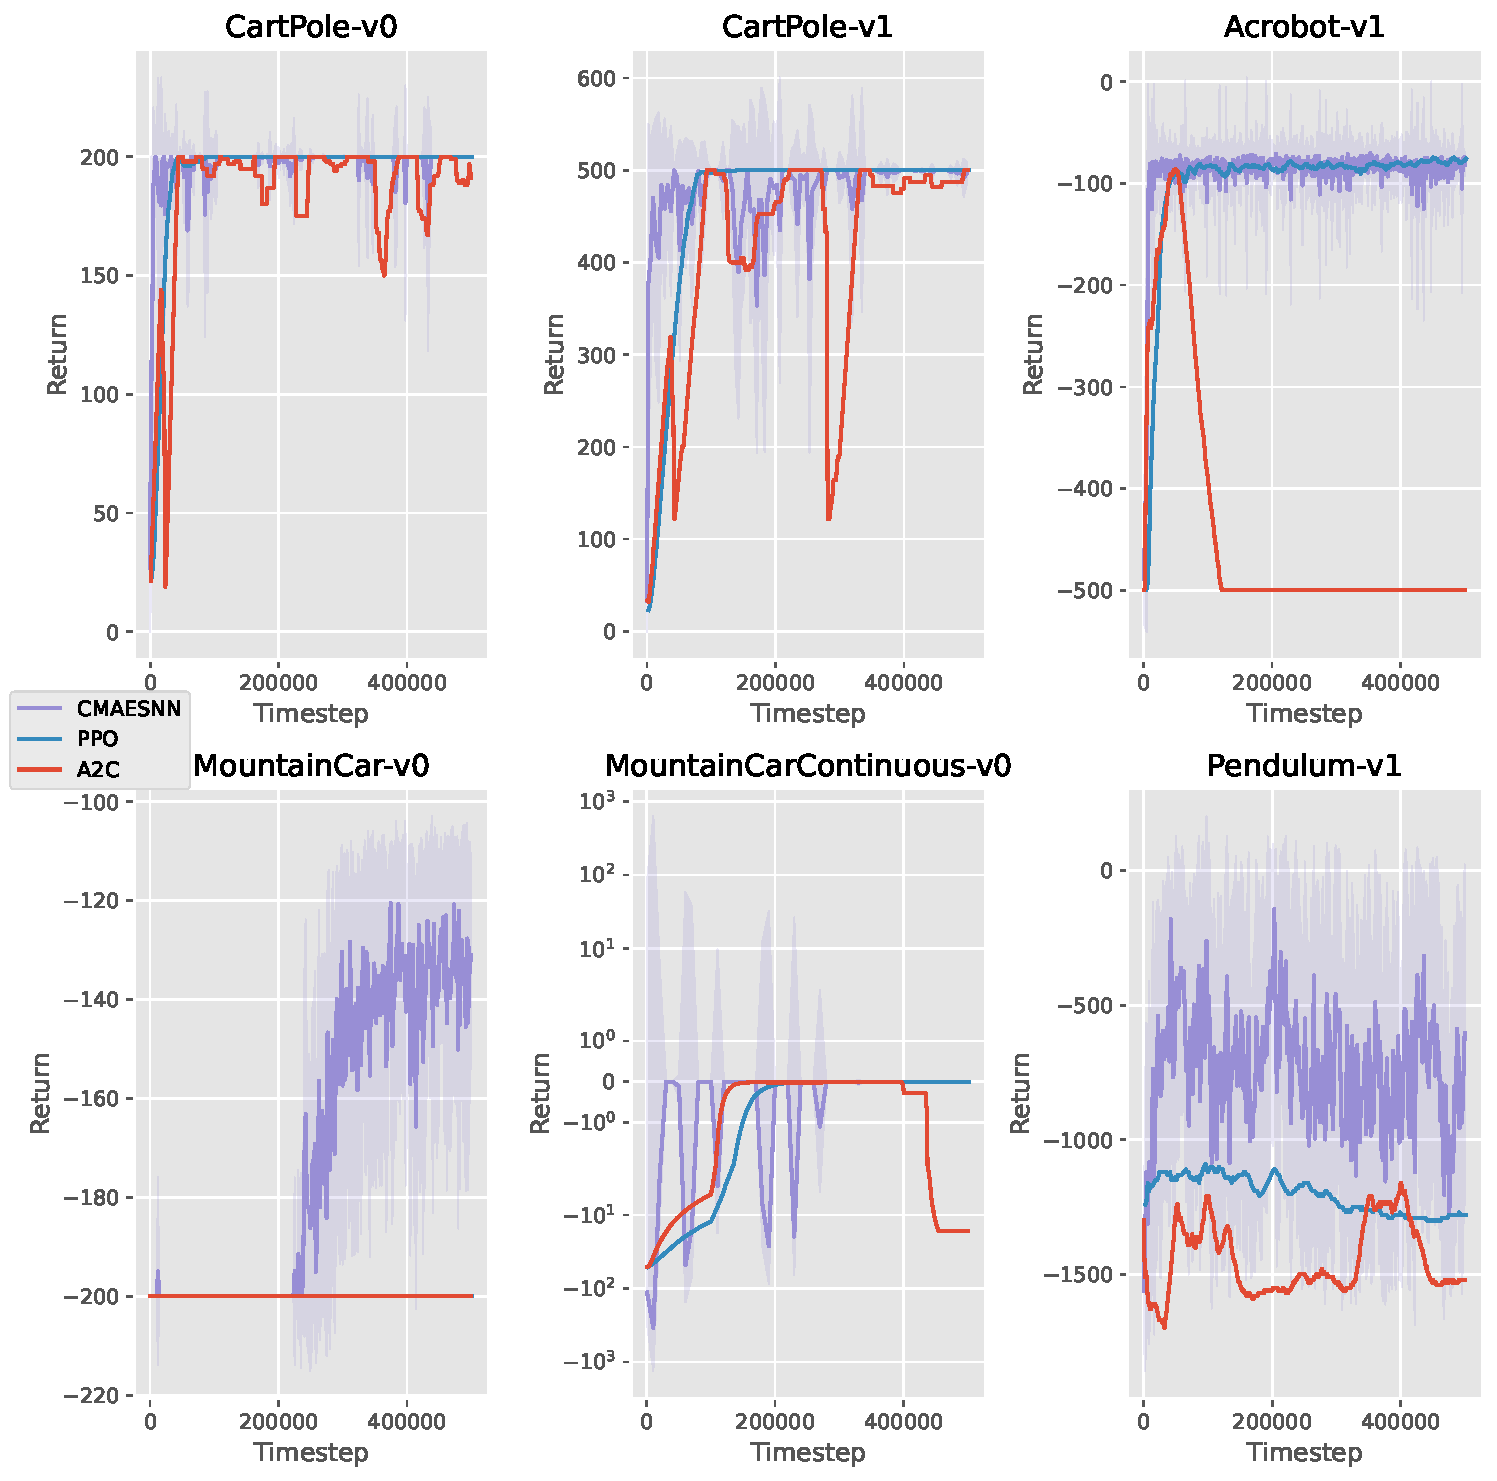
\includegraphics[width=\textwidth]{../plotting/plots/plot_all2.pdf}
    \caption{}
  \end{subfigure}
  \hspace{0.05\textwidth}
  \begin{subfigure}[ht!]{0.35\textwidth}
    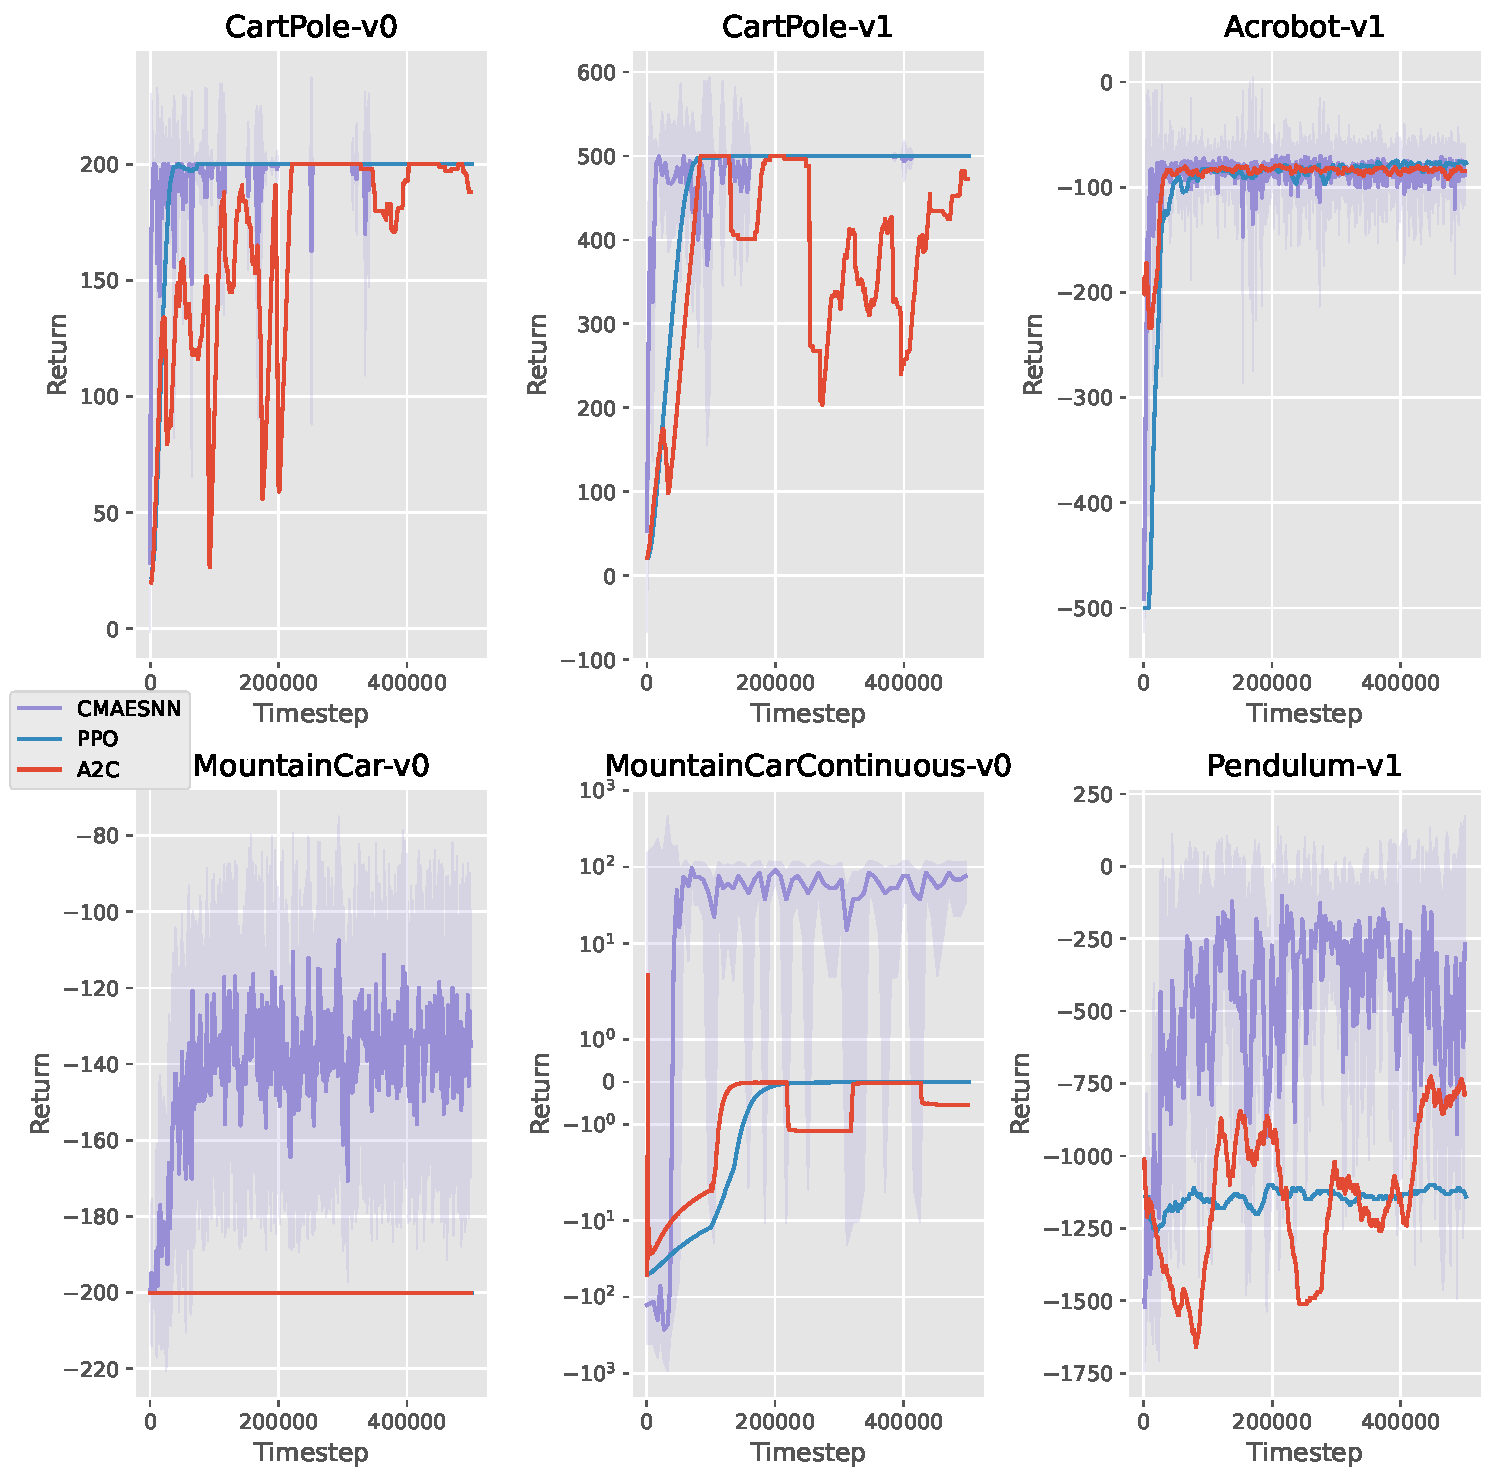
\includegraphics[width=\textwidth]{../plotting/plots/plot_all3.pdf}
    \caption{}
  \end{subfigure}

  \begin{subfigure}[ht!]{0.35\textwidth}
    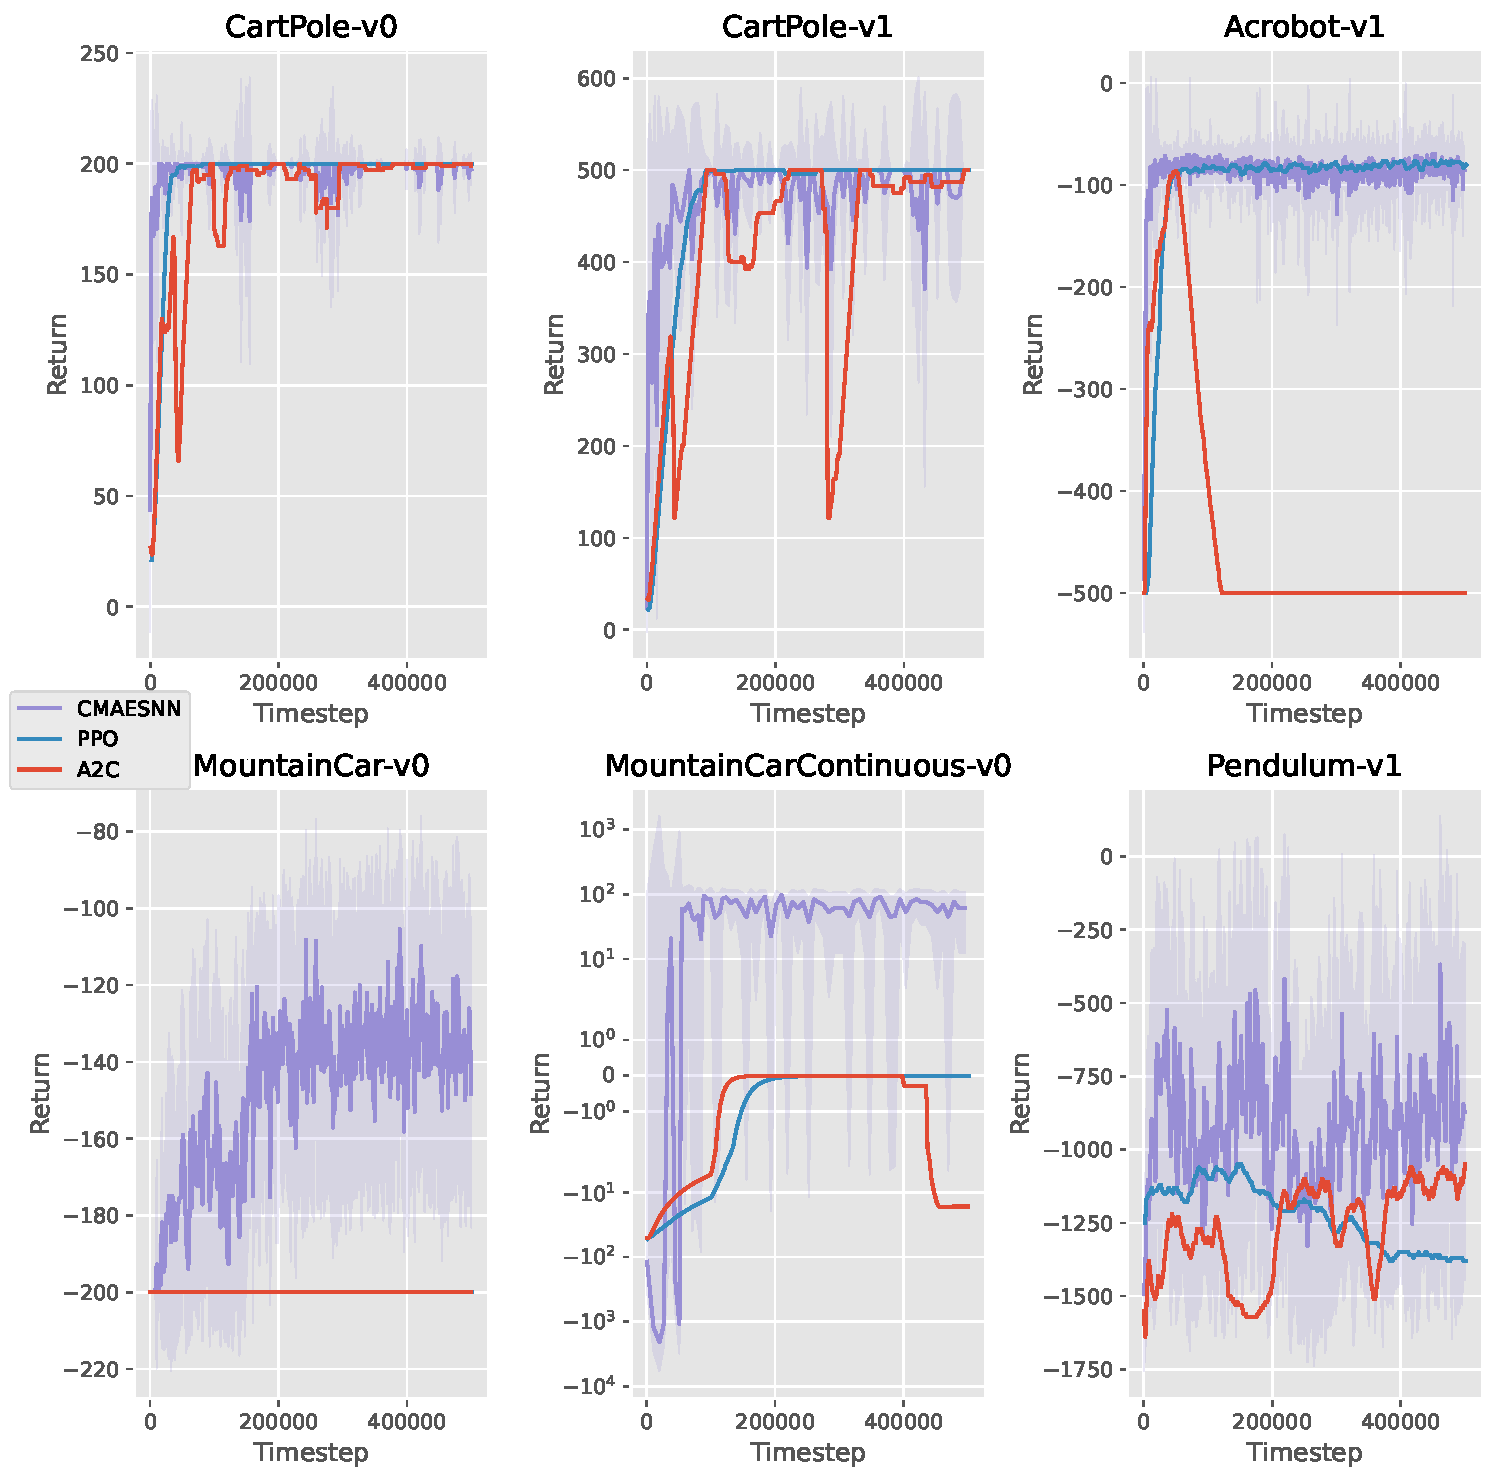
\includegraphics[width=\textwidth]{../plotting/plots/plot_all4.pdf}
    \caption{}
  \end{subfigure}
  \caption{Pięć niezależnych przebiegów uczenia algorytmów w przeciągu 500,000 kroków.
    Algorytmom tym odpowiadają kolory: CMAESNN - fioletowy, PPO - niebieski,
    A2C - czerwony.}
  \label{}

\end{figure}

\pagebreak
\section{Wpływ bias'u na uczenie CMAESNN}

\begin{figure}[ht!]
  \centering
  \begin{subfigure}[ht!]{0.35\textwidth}
    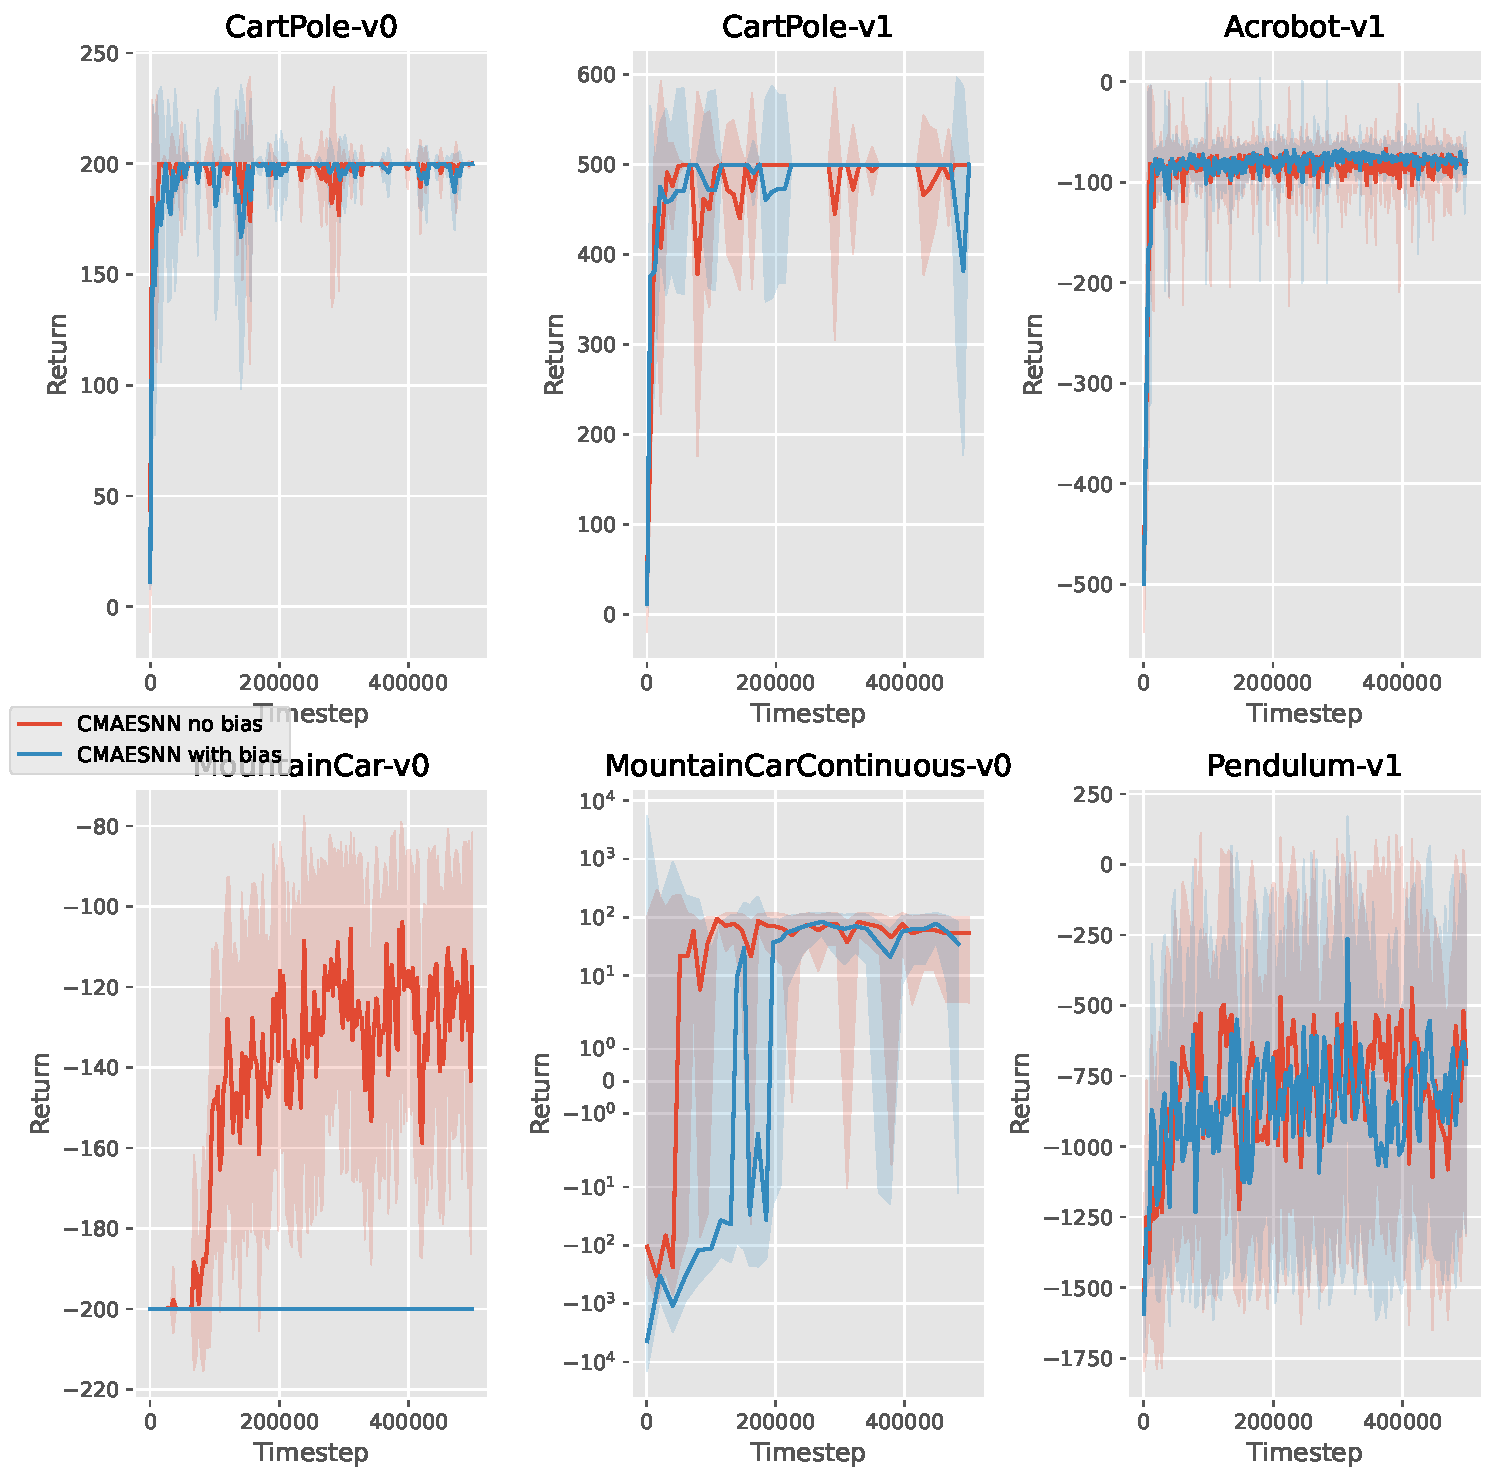
\includegraphics[width=\textwidth]{../plotting/plots/plot_bias_perf0.pdf}
    \caption{}
  \end{subfigure}
  \hspace{0.05\textwidth}
  \begin{subfigure}[ht!]{0.35\textwidth}
    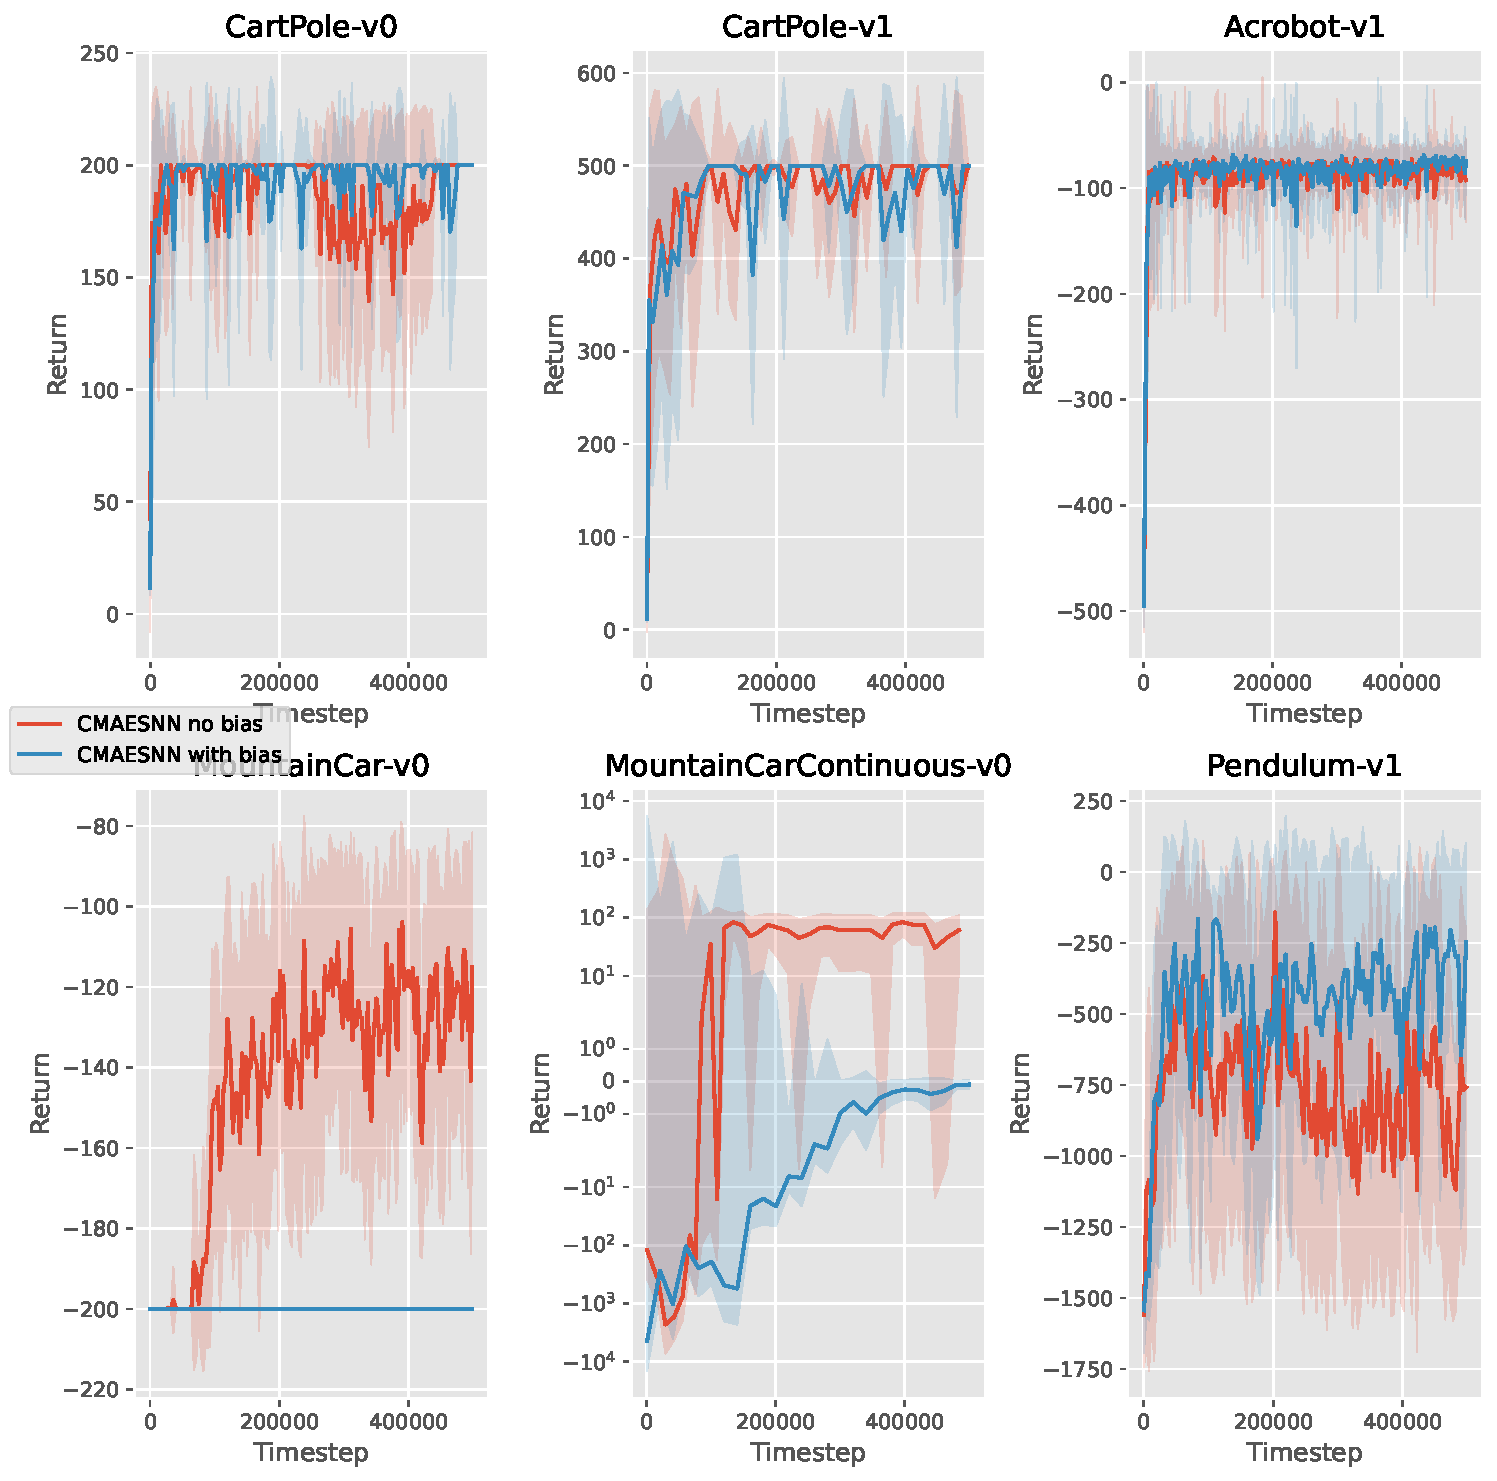
\includegraphics[width=\textwidth]{../plotting/plots/plot_bias_perf1.pdf}
    \caption{}
  \end{subfigure}

  \begin{subfigure}[ht!]{0.35\textwidth}
    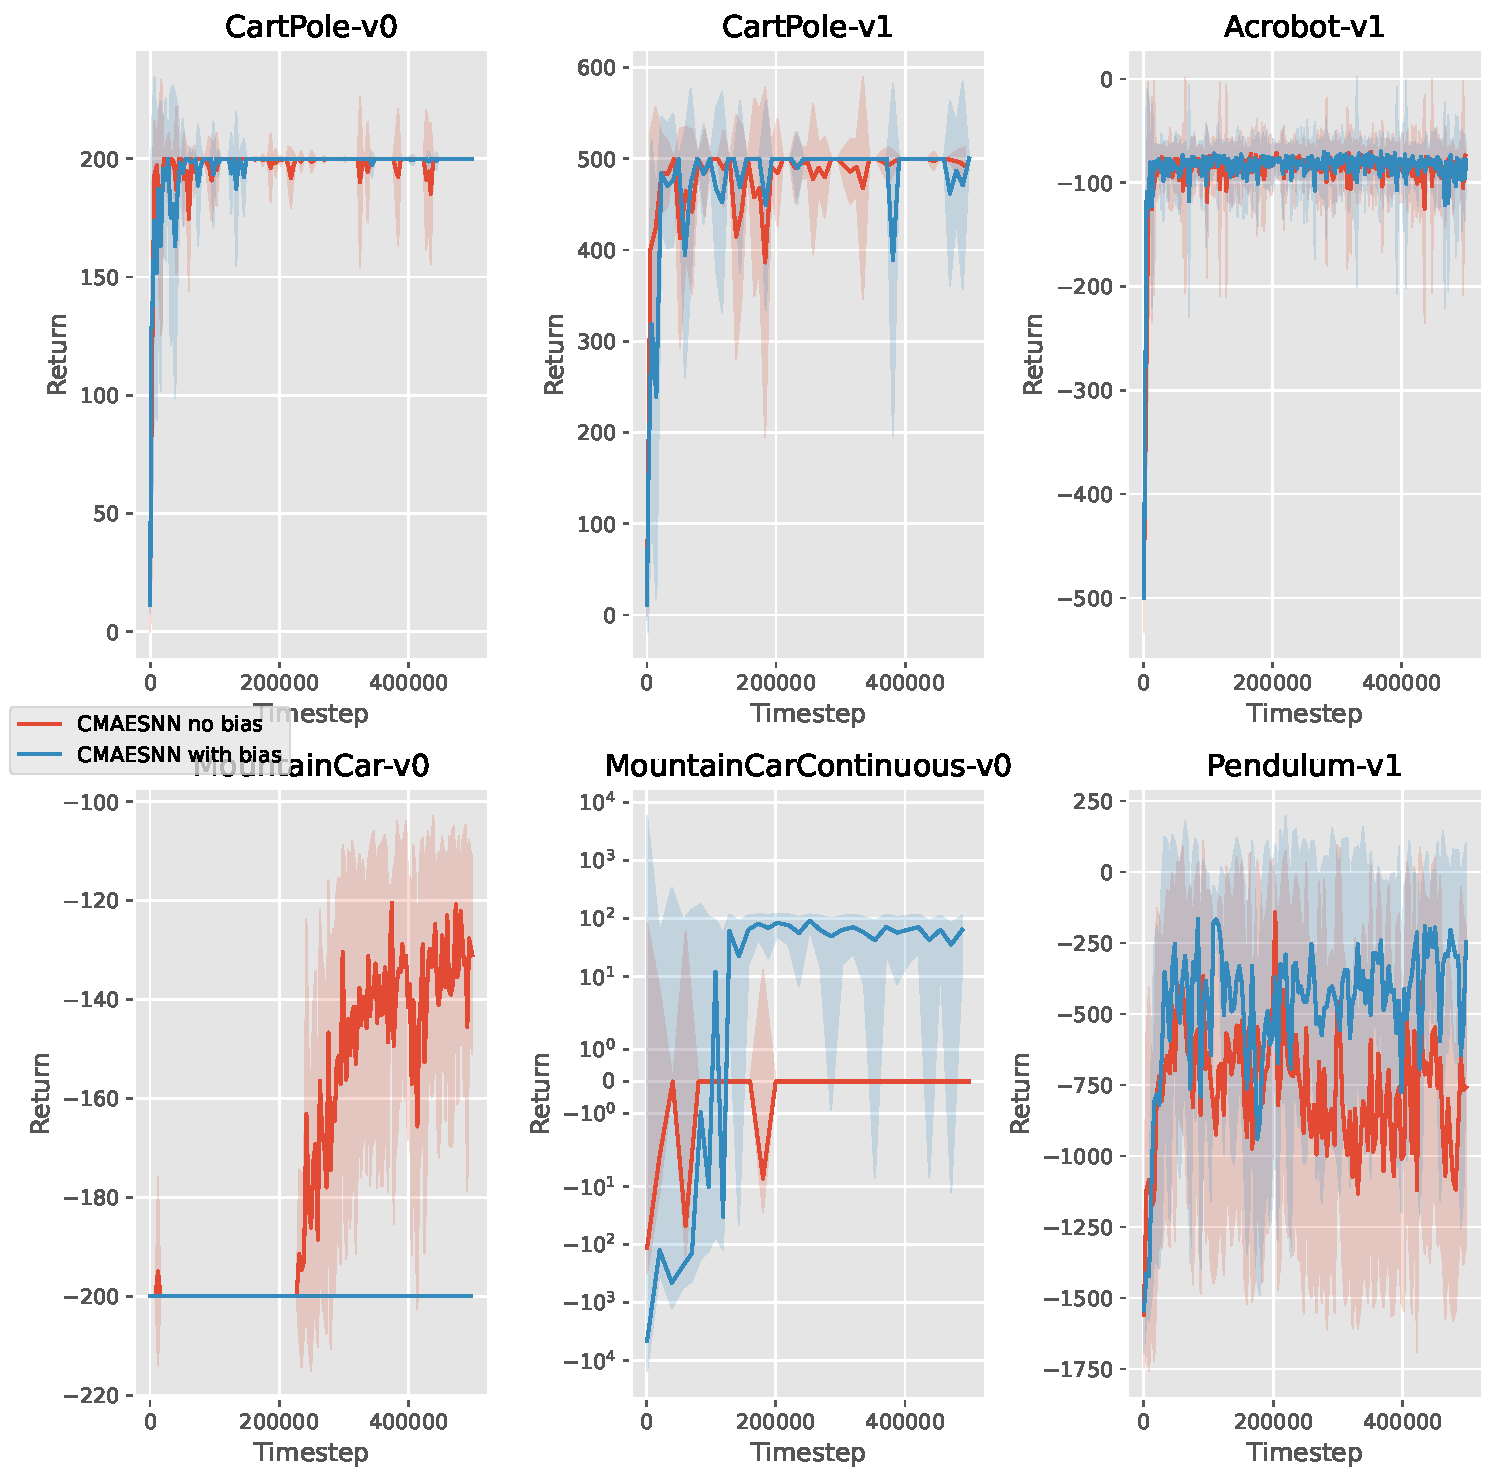
\includegraphics[width=\textwidth]{../plotting/plots/plot_bias_perf2.pdf}
    \caption{}
  \end{subfigure}
  \hspace{0.05\textwidth}
  \begin{subfigure}[ht!]{0.35\textwidth}
    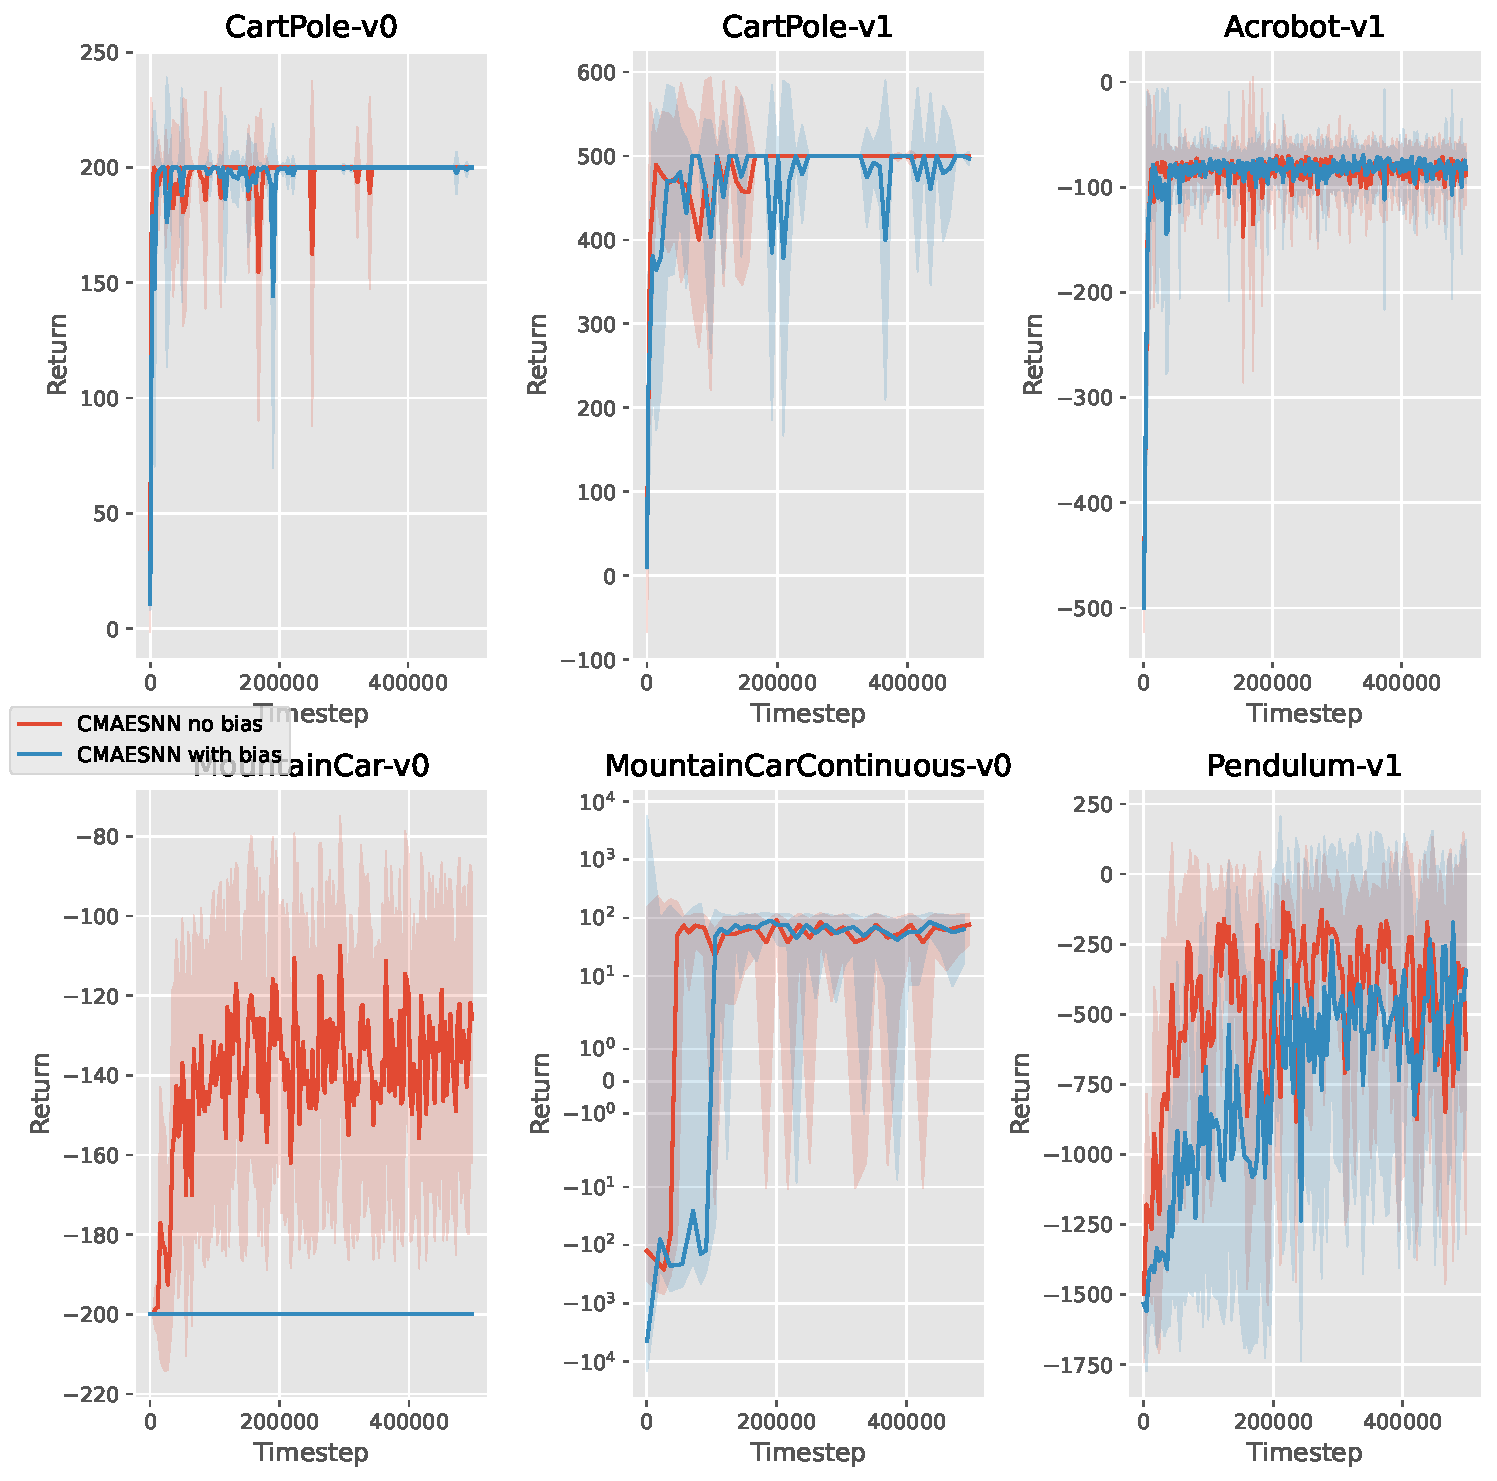
\includegraphics[width=\textwidth]{../plotting/plots/plot_bias_perf3.pdf}
    \caption{}
  \end{subfigure}

  \begin{subfigure}[ht!]{0.35\textwidth}
    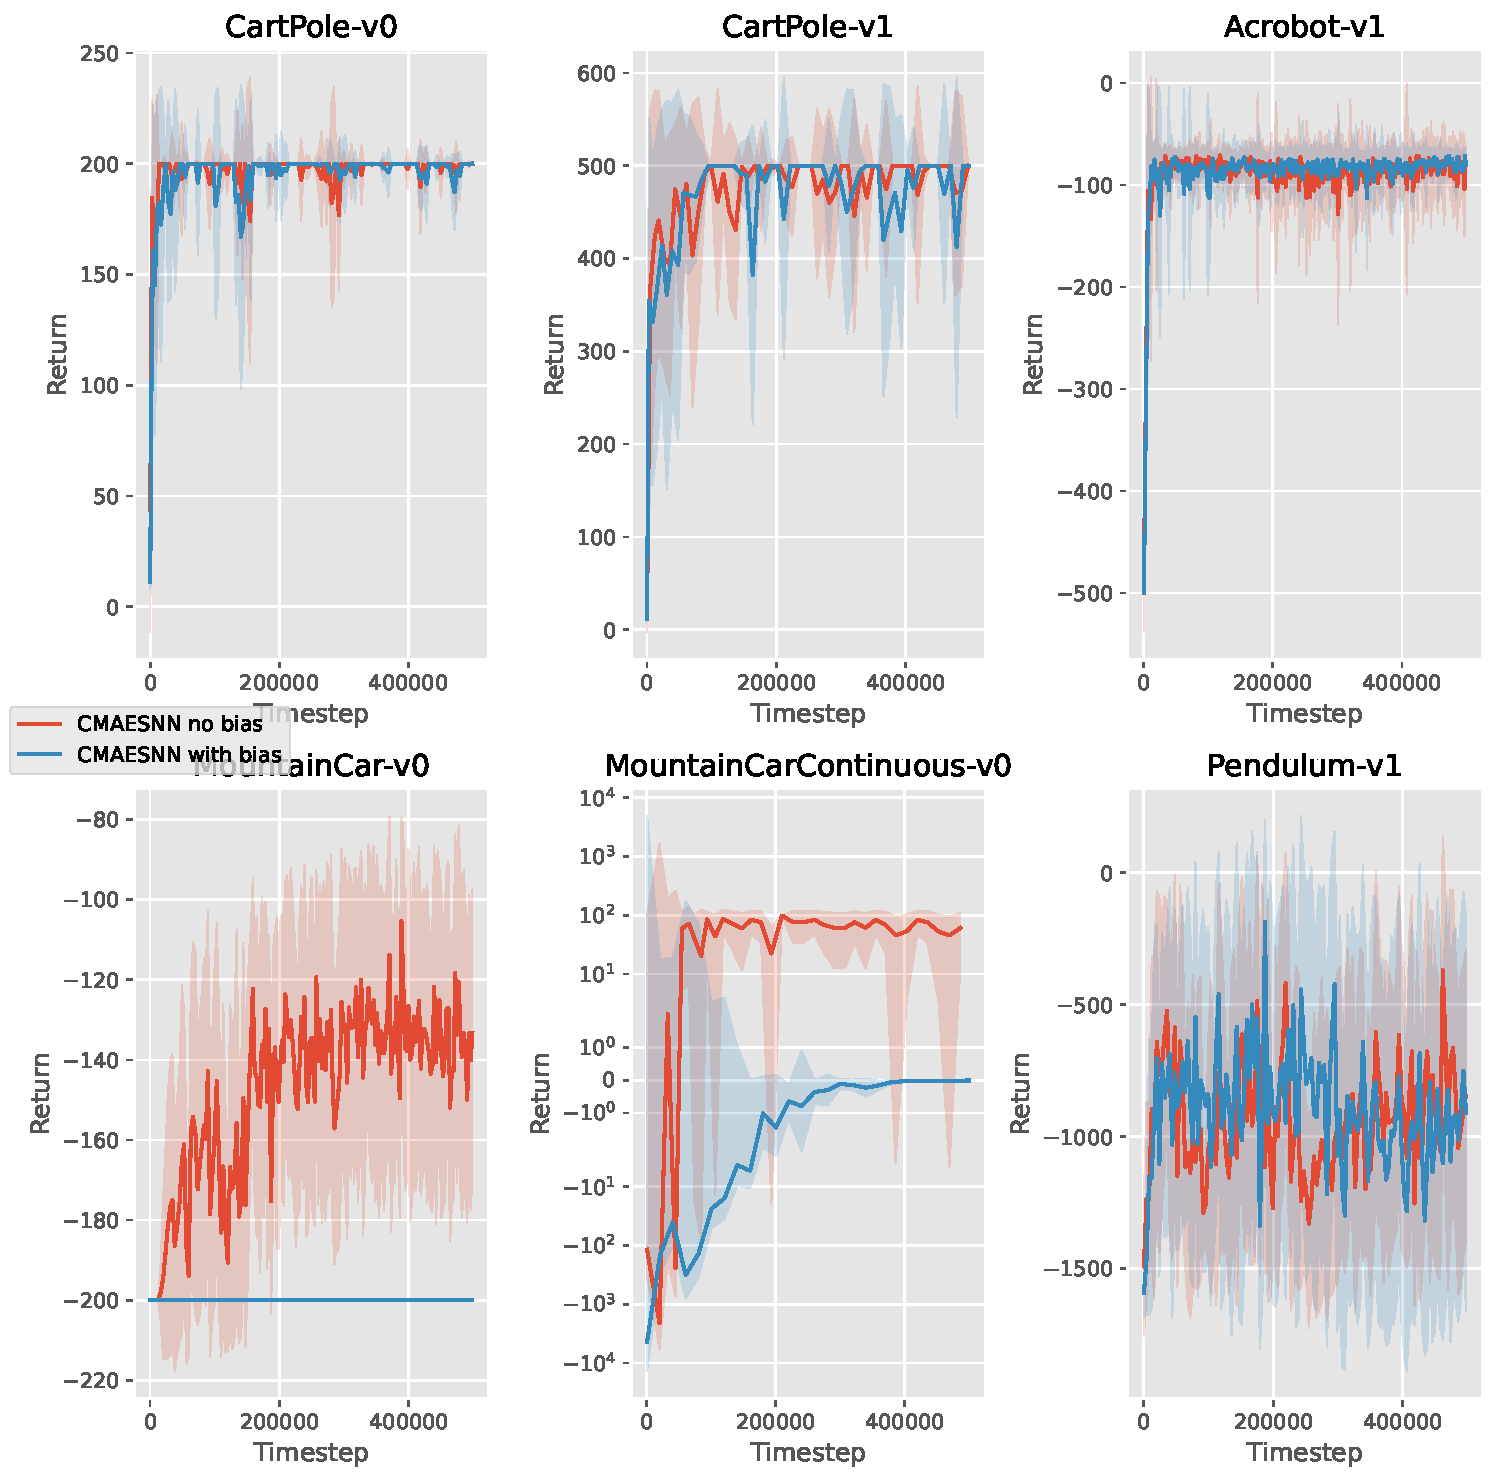
\includegraphics[width=\textwidth]{../plotting/plots/plot_bias_perf4.pdf}
    \caption{}
  \end{subfigure}
  \caption{Pięć niezależnych przebiegów uczenia algorytmów CMAESNN
    z (niebieski) i bez (czerwony) dodatkowymi parametrami bias.
    Uczenie dokonywało się w przeciągu 500,000 kroków.}
  \label{}

\end{figure}

\end{document}
